\setchapterpreamble[u]{\margintoc}
\chapter{介绍}
\labch{intro}

声明:本课题的研究秉承开源的理念,除Apple HomeKit相关项目(商用软件)外,本课题所选择的操作系统、应用程式均为开放源码软件系统。另,本课题中设计的硬件电路等设备也均开源。

\section{研究背景}
\setlength\parindent{2em} 信息技术的不断发展,催生出一个新的概念——物联网(Internet of Things, IoT)\sidenote[][90mm]{The Internet of things (IoT) is a system of interrelated computing devices, mechanical and digital machines provided with unique identifiers (UIDs) and the ability to transfer data over a network without requiring human-to-human or human-to-computer interaction.}。即将生活中原本须手动操作的物品接入网路,以实现自动化、智能化、集中化的管理与操控。在这种情况下,各大互联网厂商都对此提出过或多或少的物联网解决方案。可以说,它已经深入到了人们的生活中。
\par 众多物联网产品中——大概是由于产品定位或专利等影响吧——普遍地价格很高,哪怕是一个简单的遥控灯泡,也要数十元钱;想把它们带到日常生活中去使用,可不是一件简单的事情——至少我是这么认为的。
\par 于是,如何用更低的成本达到相同甚至更好的效果,就是我要去思考与研究的了,问题由此产生。

\section{研究大致流程}
\par 众多物联网设备中,应用最广泛的应该是智能开关、智能灯泡等基础生活用电器;对于这些设备甚至更复杂的设备,其核心在于通过网络控制其工作状态。换句话说,大部分设备中不可缺少的部分,就是一个由网络控制的开关电路。这,也就是我们要设计的对象。
\par 本课题将从思路的提出开始,对硬件、电路的选材、设计、部署等;对软件及应用程式的适配、编译、烧录等步骤进行操作与记录;以达到在实践中研究、在研究中学习的目的。

\section{研究目的} 
\begin{itemize}
	\item 了解物联网最新发展情况
	\item 利用电学与信息技术学等知识,设计、制造、部署自己的物联网设备
	\item 开拓思路,寻找与设计更优秀的解决方案
	\item ……
\end{itemize}

\section{有关技术}
\begin{itemize}
	\item 基础PCB印刷线路板的设计
	\item 微型控制单元(单片机)、微型计算机等相关知识
	\item 底层程式设计
	\item 无线网络有关软硬件知识
	\item ……
\end{itemize}

\begin{marginfigure}[1.5cm]
	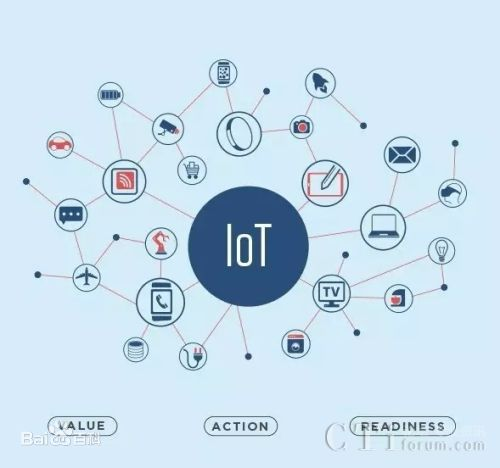
\includegraphics{iot}
	\caption[iot]{The IoT.\\ 
	\url{https://bkimg.cdn.bcebos.com/pic/562c11dfa9ec8a13e355fe69f903918fa1ecc0e8?x-bce-process=image/watermark,image_d2F0ZXIvYmFpa2U4MA==,g_7,xp_5,yp_5}}
\end{marginfigure}

